\documentclass[10pt]{article}
\usepackage{icmlko}

\icmlmeta{IP 파운데이션 월드모델}{167}{이력이 아니라 표본에 든 적이 있는가였다}{펀딩만 왜 음수인지 물었더니 펀딩만 제대로 세고 있었다 --- 나머지 일곱은 ``이전 작품 수''가 아니라 ``전에도 우리 표본에 들었나''를 재고 있었다}

\begin{document}

\twocolumn[
\icmlheader

\begin{abstract}
노트 166이 제작사 이력 축을 여덟 도메인에서 7/8 · 8/8 로 확인하고 ``펀딩만
음수($-$0.207) --- 창작자가 많을수록 나쁜가''를 남겼다. 먼저 시간 대리를
의심했다. \textbf{아니다} --- 유보 창 안에서 이 축과 날짜의 상관이 평균
$-$0.045이고, 날짜를 통제해도 라벨 상관이 $+$0.085에서 $+$0.066으로 거의
안 변한다. 그다음 펀딩의 수치를 직접 재현하려다 안 맞았다. 내가 다시 센
값과 모듈 값의 상관이 \textbf{$+$0.452}밖에 안 된다(다른 도메인은
0.97$\sim$1.00). 이유를 찾았다 --- \textbf{펀딩만 외부 전수 색인으로
센다}(\texttt{funding\_creators.py}, 와디즈 3,876쪽을 긁어 만든 창작자
색인). 나머지 일곱은 \emph{우리 표본 안에서} 같은 주체의 앞선 레코드를
센다. \textbf{둘은 다른 물건이다.} 표본 안 계수에서 ``0건''은 ``처음 만든
창작자''가 아니라 \textbf{``전에는 우리 표본에 없던 창작자''}다. 그리고
우리 표본은 도메인마다 인기 상위로 걸러져 있다. 그래서 갈라 봤다.
\textbf{효과가 통째로 0 대 1$+$ 점프다} --- 여섯 도메인에서 0건 대 1건
이상의 상관이 6/6 양수(평균 $+$0.132)인데, \textbf{1건 이상 안에서의
기울기는 4/6에 평균 $-$0.015로 없다.} 1건이든 3건이든 차이가 없다.
\textbf{즉 이 축은 ``얼마나 많이 만들었나''가 아니라 ``전에도 한 번
들었나''라는 이진 표지다.} 그리고 전수로 센 유일한 도메인에서 부호가
음수다 --- 펀딩을 표본 안 계수로 다시 세면 $-$0.005(카테고리 통제 뒤
$+$0.077)로 점프가 사라지고, 전수 색인으로는 $-$0.207이다.
\textbf{노트 166의 8/8은 창작자 이력이 아니라 표본 선택을 재고 있었을
공산이 크다.} 축이 쓸모없다는 말은 아니다 --- ``전에 히트를 낸 창작자인가''
는 오픈 전에 알 수 있는 진짜 정보다. 다만 \textbf{이름과 손잡이 해석이
틀렸다.} 기획자가 돌릴 수 있는 손잡이는 ``작품 수를 늘린다''가 아니라
``이력 있는 창작자를 쓴다''이고, 그건 켜고 끄는 스위치지 눈금이 아니다.
\end{abstract}
]

\begin{figure*}[t]
\centering
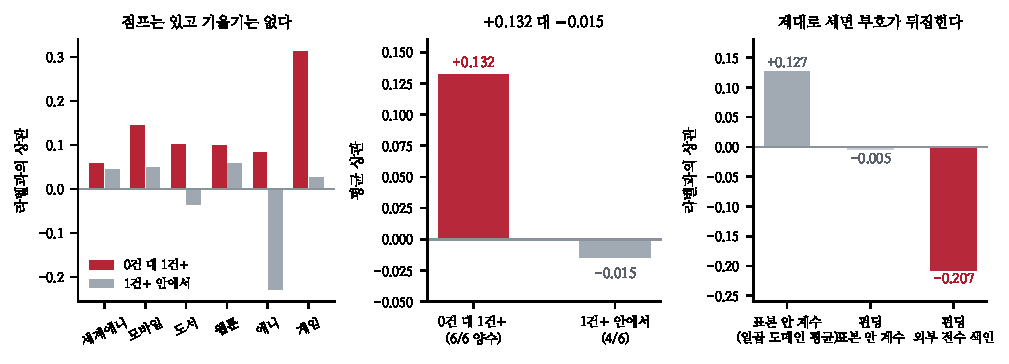
\includegraphics[width=\textwidth]{figs/member.pdf}
\caption{왼쪽 --- 점프는 있고 기울기는 없다. 가운데 --- $+$0.132 대
$-$0.015. 오른쪽 --- 제대로 세면 부호가 뒤집힌다.}
\end{figure*}

\section{시간 대리는 아니다}

축이 ``표본 안 앞선 레코드 수''이므로 날짜와 구조적으로 엮인다. 먼저 그것을
쟀다.

\begin{table}[t]
\centering\tsize
\caption{유보 창(2025$+$) 안에서.}
\begin{tabular}{lrr}
\toprule
& 날짜와 상관 & 라벨 상관 \\
\midrule
평균 & $-$.045 & $+$.085 \\
날짜 통제 뒤 & --- & $+$.066 \\
\bottomrule
\end{tabular}
\end{table}

\claimx{\textbf{시간 대리가 아니다.} 유보 창은 1년 반이라 그 안에서는
사전작 수가 거의 안 늘어난다 --- 날짜와의 상관이 $-$0.045다.}{전체 기간으로
보면 다르다. 구조상 초기 레코드는 사전작이 0일 수밖에 없다. 유보 창만
쓰는 이 판에서는 문제가 안 된다.}

\section{재현이 안 맞았다}

\begin{table}[t]
\centering\tsize
\caption{내가 다시 센 값과 모듈 값의 상관.}
\begin{tabular}{lr}
\toprule
만화 & $+$.997 \\
세계애니 & $+$.987 \\
모바일 & $+$.981 \\
도서 & $+$.974 \\
\textbf{펀딩} & \textbf{$+$.452} \\
\bottomrule
\end{tabular}
\end{table}

\claimx{\textbf{펀딩만 다르게 센다.} \texttt{ingest/funding\_creators.py}
가 와디즈 3,876쪽을 긁어 창작자 색인을 만들고, 모듈은 그 \emph{전수} 로
사전 프로젝트를 센다. 나머지 일곱은 우리 표본 400$\sim$2,948건 \emph{안에서}
센다.}{펀딩 쪽이 옳은 측정이다. 노트 22에서 와디즈 API 의 창작자 필터가
작동하지 않아 색인을 따로 만든 이력이 있다 --- 그 수고가 이 축을 유일하게
제대로 만들었다.}

\claimx{\textbf{그러면 ``0건''의 뜻이 다르다.} 전수에서는 ``처음 만든
창작자''이고, 표본 안 계수에서는 \textbf{``전에는 우리 표본에 없던
창작자''} 다. 우리 표본은 도메인마다 인기 상위로 걸러져 있다.}{웹툰은
거의 전수에 가깝지만 게임은 스팀 십수만 중 482건이다. \textbf{게임의 효과가
$+$0.312로 제일 큰 것이 그 방향과 맞는다} --- 인과 주장은 아니고 관측이다.}

\section{점프는 있고 기울기는 없다}

\begin{table}[t]
\centering\tsize
\caption{0건 대 1건 이상, 그리고 1건 이상 안에서.}
\begin{tabular}{lrrr}
\toprule
& 0건 비율 & 0 대 1$+$ & 1$+$ 안에서 \\
\midrule
게임 & 57.0\% & \textbf{$+$.312} & $+$.026 \\
모바일 & 58.3\% & \textbf{$+$.143} & $+$.048 \\
도서 & 47.2\% & $+$.101 & $-$.035 \\
웹툰 & 47.8\% & $+$.097 & $+$.059 \\
애니 & 81.8\% & $+$.083 & \textbf{$-$.229} \\
세계애니 & 5.3\% & $+$.058 & $+$.044 \\
\midrule
\textbf{평균} & & \textbf{$+$.132} & \textbf{$-$.015} \\
\bottomrule
\end{tabular}
\end{table}

\claimx{\textbf{효과가 통째로 이진 점프다.} 0건 대 1건 이상이 6/6 양수에
평균 $+$0.132인데, 1건 이상 안에서의 기울기는 4/6에 평균 $-$0.015다.
\textbf{1건이든 3건이든 차이가 없다.}}{``1건 이상''의 표본이 도메인마다
100$\sim$280건이라 기울기 추정의 오차가 크다. 다만 여섯 중 넷만 양수이고
평균이 0이라는 것은 ``기울기가 있는데 못 봤다''로 읽기 어렵다.}

\claimx{\textbf{그러니 이 축은 눈금이 아니라 스위치다.} ``전에도 우리
표본에 든 창작자인가''라는 이진 표지이고, 우리 표본이 인기 상위라면 그것은
\textbf{``전에 히트를 낸 적 있나''} 다.}{그것 자체는 오픈 전에 알 수 있는
진짜 정보다 --- 라벨 누수가 아니다. 이 작품의 결과가 아니라 \emph{이전
작품들의} 결과로 정해지니까.}

\section{전수로 세면 부호가 뒤집힌다}

\begin{table}[t]
\centering\tsize
\caption{펀딩. 같은 도메인, 세는 법만 다르다.}
\begin{tabular}{lr}
\toprule
표본 안 계수 (내가 다시 셈) & $-$.005 \\
\quad 카테고리 통제 뒤 & $+$.077 \\
\textbf{외부 전수 색인 (모듈)} & \textbf{$-$.207} \\
\bottomrule
\end{tabular}
\end{table}

\claimx{\textbf{표본 안으로 세면 점프가 사라진다} --- 펀딩 유보 80건 중
0건이 65건이고 0 대 1$+$ 차이가 라벨 중앙 1.959 대 1.924로 없다. 펀딩
표본은 인기 필터가 약하다는 뜻이다.}{펀딩은 400건이고 와디즈 전체는
훨씬 크다. 그런데도 점프가 없는 것은 이 표본의 뽑기가 성과 기준이 아니었을
수 있다 --- 그렇다면 다른 도메인의 점프가 더 의심스러워진다.}

\claimx{\textbf{그리고 전수로는 음수다}($-$0.207). 창작자의 실제 프로젝트
이력이 많을수록 후원자가 적다.}{크라우드펀딩만의 성질일 수 있다 --- 첫
캠페인이 플랫폼 추천과 신선함을 받는다. 도메인 하나짜리 관측이라 일반화는
못 한다.}

\section{그래서 노트 166을 고친다}

\claimx{\textbf{노트 166의 7/8 · 8/8 은 창작자 이력이 아니라 표본 선택을
재고 있었을 공산이 크다.} 여덟 칸 중 일곱이 표본 안 계수이고, 그 효과가
전부 0 대 1$+$ 점프다.}{축을 버리자는 것이 아니다. \textbf{이름과 손잡이
해석을 고쳐야 한다} --- 기획자가 돌릴 수 있는 것은 ``작품 수를 늘린다''가
아니라 ``이력 있는 창작자를 쓴다''이고, 그건 스위치지 눈금이 아니다.}

\begin{table}[t]
\centering\tsize
\caption{남은 것.}
\begin{tabular}{ll}
\toprule
\textbf{전수 색인} & 다른 도메인도 만들면 --- 게임은 스팀 API \\
표본 필터 & 도메인마다 어떻게 뽑았나 --- 문서가 없다 \\
스위치 축 & 이진으로 다시 만들면 판이 어떻게 되나 \\
\bottomrule
\end{tabular}
\end{table}

첫 줄이 값비싸고 둘째 줄이 값싸다. \textbf{도메인마다 표본을 어떻게
뽑았는지가 어디에도 안 적혀 있다} --- 인기 상위 $N$ 인지 전수인지에 따라
이 축의 뜻이 통째로 바뀌는데도. 그것부터 적는 것이 다음이다.

\end{document}
